%%%%%%%%%%%%%%%%%%%%%%%VICARIOUS%%%%%%%%%%%%%%%%%%%%%%%%%%%%%%%%%%%%%%%
% Copyright ME, FUCK YOU			      		      %
% Template for presentation in Latex`s Beamer Class		      %
% Using the default Berlin theme, can be replaced by other themes     %
% logo in the upper right can be replaced by new .png, gif, eps etc   %
% 								      %
%%%%%%%%%%%%%%%%%%%%%%%%%%%%%%%%%%%%%%%%%%%%%%%%%%%%%%%%%%%%%%%%%%%%%%%
\documentclass[xcolor=dvipsnames]{beamer}
\usetheme{Berlin}
\usecolortheme[named=LimeGreen]{structure}
\usepackage{beamerthemesplit} % kam neu dazu
\usepackage[ngerman]	{babel}			
\usepackage{t1enc}						
\usepackage[utf8]{inputenc}			
\usepackage{amsmath}
\usepackage{graphicx}
\graphicspath{{pictures/}}
\usepackage{amssymb}
\usepackage{amsfonts}
\usepackage{caption}
\usepackage{multimedia}
\usepackage{tikz}
\usepackage{listings}
\usepackage{acronym}

\usepackage{lmodern}
\usepackage{multicol}


\definecolor{pblue}{rgb}{0.13,0.13,1}
\definecolor{pgreen}{rgb}{0,0.5,0}
\definecolor{pred}{rgb}{0.9,0,0}
\definecolor{pgrey}{rgb}{0.46,0.45,0.48}

\lstset{
    escapeinside={(*}{*)}
}

\lstdefinestyle{Java}{
  showspaces=false,
  showtabs=false,
  tabsize=2,
  breaklines=true,
  showstringspaces=false,
  breakatwhitespace=true,
  commentstyle=\color{pgreen},
  keywordstyle=\color{pblue},
  stringstyle=\color{pred},
  basicstyle=\footnotesize\ttfamily,
  numbers=left,
  numberstyle=\tiny\color{gray}\ttfamily,
  numbersep=7pt,
  %moredelim=[il][\textcolor{pgrey}]{$$},
  moredelim=[is][\textcolor{pgrey}]{\%\%}{\%\%},
  captionpos=b
}

\lstdefinestyle{basic}{  
  basicstyle=\footnotesize\ttfamily,
  breaklines=true
  numbers=left,
  numberstyle=\tiny\color{gray}\ttfamily,
  numbersep=7pt,
  backgroundcolor=\color{white},
  showspaces=false,
  showstringspaces=false,
  showtabs=false,
  frame=single,
  rulecolor=\color{black},
  captionpos=b,
  keywordstyle=\color{blue}\bf,
  commentstyle=\color{gray},
  stringstyle=\color{green},
  keywordstyle={[2]\color{red}\bf},
}


\lstdefinelanguage{custom}
{
morekeywords={public, void},
sensitive=false,
morecomment=[l]{//},
morecomment=[s]{/*}{*/},
morestring=[b]",
}


\lstdefinestyle{BashInputStyle}{
  language=bash,
  showstringspaces=false,
  basicstyle=\small\sffamily,
  numbers=left,
  numberstyle=\tiny,
  numbersep=5pt,
  frame=trlb,
  columns=fullflexible,
  backgroundcolor=\color{gray!20},
  linewidth=0.9\linewidth,
  xleftmargin=0.1\linewidth
}

%Logo in the upper right just change if you know what you are doing^^
\addtobeamertemplate{frametitle}{}{%
\begin{tikzpicture}[remember picture,overlay]
\node[anchor=north east,yshift=2pt] at (current page.north east) {
\includegraphics[height=1.8cm]{htw}};
\end{tikzpicture}}

\begin{document}
\bibliographystyle{alpha}
\title{Netzwerke -- Seminaristische Übung WS17/18}
\subtitle{Wirshark \& Routing\\
		\href{mailto:Benjamin.Troester@HTW-Berlin.de}{Benjamin.Troester@HTW-Berlin.de}\\
		PGP: ADE1 3997 3D5D B25D 3F8F 0A51 A03A 3A24 978D D673 }
\author{Benjamin Tröster}

\date{\today}

\begin{frame}
\titlepage
\end{frame}

\section*{Road-Map}
\begin{frame}
\frametitle{Road-Map}
\begin{multicols}{2}
  \tableofcontents
\end{multicols}
\end{frame}

\section*{Stuff}
\begin{frame}{Nerd-Wochenmarkt}
Empfehlung der Woche:
\begin{itemize}
	\item Request for Comments -- Der RFC Podcast
	\begin{itemize}
		\item IP Routing I: \url{https://requestforcomments.de/archives/343}
		\item IP Routing II: \url{https://requestforcomments.de/archives/351}
		\item IP Routing III: \url{https://requestforcomments.de/archives/374}   
	\end{itemize}
	\item Datengarten des CCCB
	\begin{itemize}
		\item Technik und Wahrheit \url{https://media.ccc.de/v/dg-82}
	\end{itemize}
\end{itemize}
\end{frame}

\section{Orga}
\begin{frame}
	\begin{itemize}
		\item Halten Sie bitte Ordnung! D.h.:
		\begin{itemize}
			\item Räumen Sie \textbf{alle} verwendeten Geräte wieder weg
			\item Seien Sie sozial, falls Kommilitonen dies vergessen
			\item Achten Sie darauf die Raspberry Pis vorsichtig zu behandeln $\rightarrow$ Leihgabe
		\end{itemize}
		\item Versuchen Sie nicht erste 30 Minuten später zu erscheinen! 
		\item Die Zeit fehlt Ihnen am Ende der Übung
	\end{itemize}
\end{frame}

\section{Retrospektive}
\begin{frame}{Retrospektive}
\begin{itemize}
	\item Vorlesung
	\begin{itemize}
		\item Fragen?
	\end{itemize}
	\item Übungsblatt 3 -- Switched Networks
	\begin{itemize}
		\item Stand der Gruppen
		\item Fragen?
	\end{itemize}
\end{itemize}
\end{frame}

\section{Wireshark}
\begin{frame}
\centering

\includegraphics[scale=0.3]{wireshark_s}
\end{frame}

\begin{frame}
\hspace{-1.3cm}
\begin{minipage}{0.6\textwidth}
\begin{itemize}
	\item Network Sniffer - setzt auf libcap auf
	\item Erlaubt mitschneiden und auswerten des Netzwerkverkehrs
	\item \url{https://www.wireshark.org/}
	\item Doku: \url{https://www.wireshark.org/docs/wsug_html_chunked/} $\rightarrow$ ab Chpt. 3.3 wird es interessant
	\item \textbf{Heutige Übung} -- Auswertung von Ethernet-Frames!
\end{itemize}
\end{minipage}%
\begin{minipage}{0.4\textwidth}
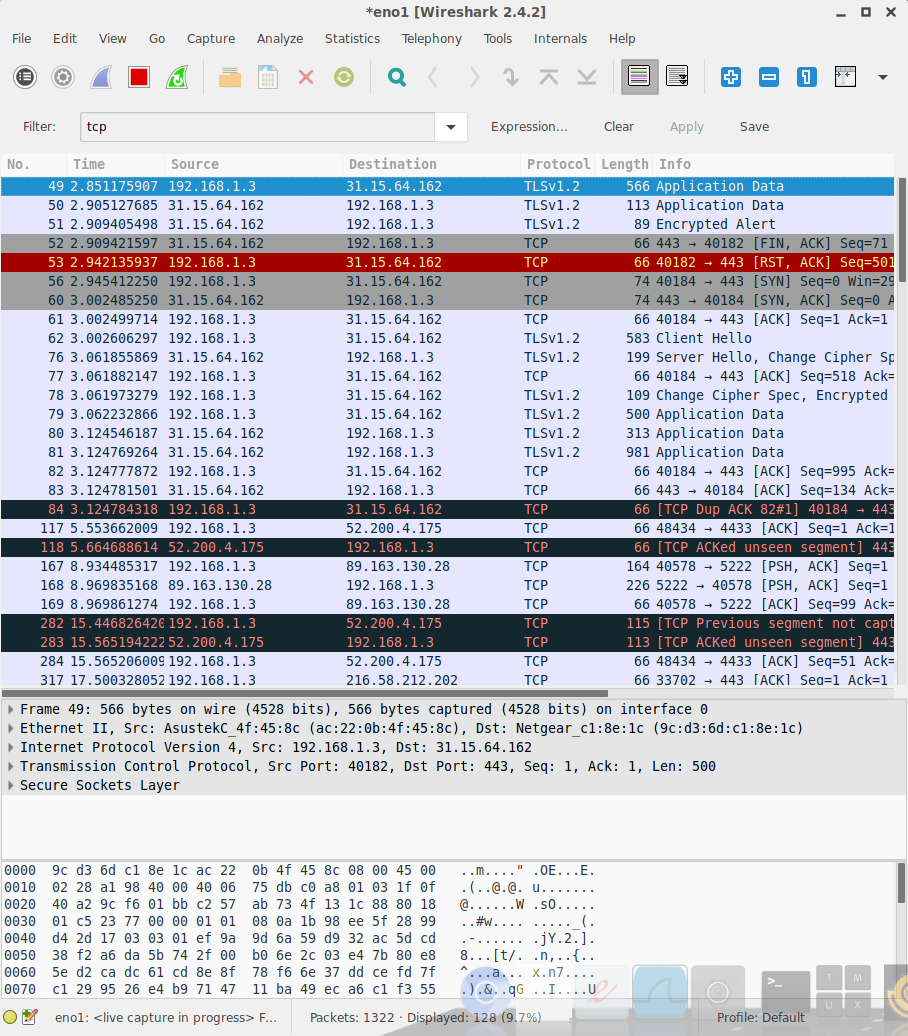
\includegraphics[scale=0.2]{wireshark}
\end{minipage}
\end{frame}

\section{Switched Networks}
\begin{frame}
	\begin{itemize}
		\item Layer 2 Devices
		\item Ethernet-Switches können (meistens) nur Ethernet-Frames versenden
		\item Zuordnung von MAC-Adressen zu IP-Adressen $\rightarrow$ erzeugen Netzwerk
	\end{itemize}
\end{frame}
\section{Routing}
\begin{frame}
	\begin{itemize}
		\item Layer 3 Device
		\item Protokoll ist wichtig!
		\item Meist IP-basiert -- d.h. IPv4/IPv6 $\rightarrow$ Routing-Protokoll
		\item \glqq Besitzen mehr Intelligenz\grqq -- mithilfe von Routing-Tabellen
		\item Verbinden Netzwerke
	\end{itemize}
\end{frame}

\begin{frame}
\vspace{-0.25cm}
\begin{figure}
\centering
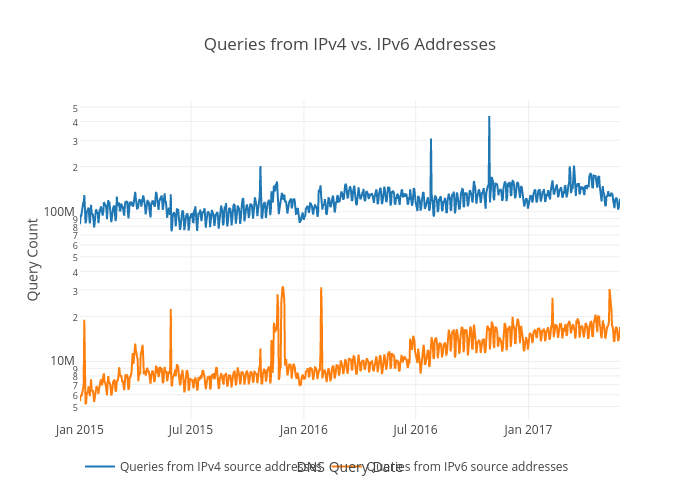
\includegraphics[scale=0.4]{ip}
\end{figure}
\end{frame}

\begin{frame}
\hspace{-1cm}
\begin{minipage}{0.6\textwidth}
\begin{itemize}
	\item Bis jetzt Switched Network
	\item Pis kennen sich über Switch
	\item kein Kommunikation über das Netz hinaus möglich
\end{itemize}
\end{minipage}%
\begin{minipage}{0.4\textwidth}
\begin{figure}
\centering
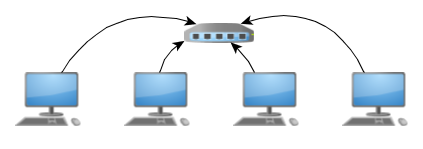
\includegraphics[scale=0.4]{current}
\end{figure}
\end{minipage}
\end{frame}

\begin{frame}
\hspace{-1cm}
\begin{minipage}{0.6\textwidth}
\begin{itemize}
	\item In dieser Übung
	\item Pis kennen sich über Gateway
	\item Kommunikation über das Netz hinaus möglich -- zwischen zwei Netzen
\end{itemize}
\end{minipage}%
\begin{minipage}{0.4\textwidth}
\begin{figure}
\centering
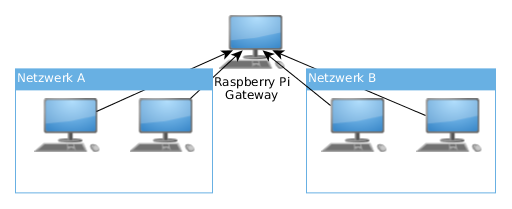
\includegraphics[scale=0.35]{gateway}
\end{figure}
\end{minipage}
\end{frame}
\end{document}